\documentclass{article}\usepackage[]{graphicx}\usepackage[]{color}
%% maxwidth is the original width if it is less than linewidth
%% otherwise use linewidth (to make sure the graphics do not exceed the margin)
\makeatletter
\def\maxwidth{ %
  \ifdim\Gin@nat@width>\linewidth
    \linewidth
  \else
    \Gin@nat@width
  \fi
}
\makeatother

\definecolor{fgcolor}{rgb}{0.345, 0.345, 0.345}
\newcommand{\hlnum}[1]{\textcolor[rgb]{0.686,0.059,0.569}{#1}}%
\newcommand{\hlstr}[1]{\textcolor[rgb]{0.192,0.494,0.8}{#1}}%
\newcommand{\hlcom}[1]{\textcolor[rgb]{0.678,0.584,0.686}{\textit{#1}}}%
\newcommand{\hlopt}[1]{\textcolor[rgb]{0,0,0}{#1}}%
\newcommand{\hlstd}[1]{\textcolor[rgb]{0.345,0.345,0.345}{#1}}%
\newcommand{\hlkwa}[1]{\textcolor[rgb]{0.161,0.373,0.58}{\textbf{#1}}}%
\newcommand{\hlkwb}[1]{\textcolor[rgb]{0.69,0.353,0.396}{#1}}%
\newcommand{\hlkwc}[1]{\textcolor[rgb]{0.333,0.667,0.333}{#1}}%
\newcommand{\hlkwd}[1]{\textcolor[rgb]{0.737,0.353,0.396}{\textbf{#1}}}%

\usepackage{framed}
\makeatletter
\newenvironment{kframe}{%
 \def\at@end@of@kframe{}%
 \ifinner\ifhmode%
  \def\at@end@of@kframe{\end{minipage}}%
  \begin{minipage}{\columnwidth}%
 \fi\fi%
 \def\FrameCommand##1{\hskip\@totalleftmargin \hskip-\fboxsep
 \colorbox{shadecolor}{##1}\hskip-\fboxsep
     % There is no \\@totalrightmargin, so:
     \hskip-\linewidth \hskip-\@totalleftmargin \hskip\columnwidth}%
 \MakeFramed {\advance\hsize-\width
   \@totalleftmargin\z@ \linewidth\hsize
   \@setminipage}}%
 {\par\unskip\endMakeFramed%
 \at@end@of@kframe}
\makeatother

\definecolor{shadecolor}{rgb}{.97, .97, .97}
\definecolor{messagecolor}{rgb}{0, 0, 0}
\definecolor{warningcolor}{rgb}{1, 0, 1}
\definecolor{errorcolor}{rgb}{1, 0, 0}
\newenvironment{knitrout}{}{} % an empty environment to be redefined in TeX

\usepackage{alltt}
\usepackage{alltt}
\usepackage{amsmath}
\usepackage[sc]{mathpazo}
\usepackage[T1]{fontenc}
\usepackage{geometry}
\geometry{verbose,tmargin=2.5cm,bmargin=2.5cm,lmargin=2.5cm,rmargin=2.5cm}
\setcounter{secnumdepth}{2}
\setcounter{tocdepth}{2}
\usepackage{url}
\usepackage[unicode=true,pdfusetitle,
 bookmarks=true,bookmarksnumbered=true,bookmarksopen=true,bookmarksopenlevel=2,
 breaklinks=false,pdfborder={0 0 1},backref=false,colorlinks=false]
 {hyperref}
\hypersetup{
 pdfstartview={XYZ null null 1}}
 
\title{Figure S3: Fixed effects framework with AR(1), block diagonal structures} 
 
\usepackage{breakurl}
\IfFileExists{upquote.sty}{\usepackage{upquote}}{}
\begin{document}
\maketitle
%\SweaveOpts{concordance=TRUE}



%Load the necessary libraries, source the file with the R functions:
\begin{knitrout}
\definecolor{shadecolor}{rgb}{0.969, 0.969, 0.969}\color{fgcolor}\begin{kframe}
\begin{alltt}
\hlkwd{library}\hlstd{(ggplot2)}
\hlkwd{library}\hlstd{(Matrix)}

\hlkwd{source}\hlstd{(}\hlstr{"functions.R"}\hlstd{)}
\end{alltt}
\end{kframe}
\end{knitrout}

Will use the same theme throughout, so just declare this variable:
\begin{knitrout}
\definecolor{shadecolor}{rgb}{0.969, 0.969, 0.969}\color{fgcolor}\begin{kframe}
\begin{alltt}
\hlstd{themeUsed} \hlkwb{<-}  \hlkwd{theme_bw}\hlstd{(}\hlkwc{base_size} \hlstd{=} \hlnum{20}\hlstd{)}\hlopt{+}
  \hlkwd{theme}\hlstd{(}\hlkwc{axis.line} \hlstd{=} \hlkwd{element_line}\hlstd{(}\hlkwc{colour} \hlstd{=} \hlstr{"black"}\hlstd{),}
        \hlkwc{plot.title} \hlstd{=} \hlkwd{element_text}\hlstd{(}\hlkwc{size} \hlstd{=} \hlnum{16}\hlstd{,} \hlkwc{hjust} \hlstd{=} \hlnum{0.5}\hlstd{),}
        \hlkwc{panel.grid.major} \hlstd{=} \hlkwd{element_blank}\hlstd{(),}
        \hlkwc{panel.grid.minor} \hlstd{=} \hlkwd{element_blank}\hlstd{(),}
        \hlkwc{panel.border} \hlstd{=} \hlkwd{element_blank}\hlstd{(),}
        \hlkwc{panel.background} \hlstd{=} \hlkwd{element_blank}\hlstd{(),}
        \hlkwc{legend.key} \hlstd{=} \hlkwd{element_blank}\hlstd{(),}
        \hlkwc{legend.text.align} \hlstd{=} \hlnum{0}\hlstd{,}
        \hlkwc{axis.line.x} \hlstd{=} \hlkwd{element_line}\hlstd{(}\hlkwc{color}\hlstd{=}\hlstr{"black"}\hlstd{,} \hlkwc{size} \hlstd{=} \hlnum{0.5}\hlstd{),} \hlcom{##this is to show axes - bug in this version of ggplot2}
        \hlkwc{axis.line.y} \hlstd{=} \hlkwd{element_line}\hlstd{(}\hlkwc{color}\hlstd{=}\hlstr{"black"}\hlstd{,} \hlkwc{size} \hlstd{=} \hlnum{0.5}\hlstd{))}
\end{alltt}
\end{kframe}
\end{knitrout}
  

\section{AR(1) correlation matrices}

These results are for the $I=2, p\ge 2$ autoregressive case with AR(1) with equal within-study variances,
so the parameters we vary are: $r, \rho_1, \rho_2, p$. 
We save the relative efficiencies for only one of coefficients, as they are all equal.
We consider $\rho_1 = 0$.
\begin{knitrout}
\definecolor{shadecolor}{rgb}{0.969, 0.969, 0.969}\color{fgcolor}\begin{kframe}
\begin{alltt}
\hlcom{##save results in data frame}
\hlstd{bigMat} \hlkwb{<-} \hlkwd{expand.grid}\hlstd{(}\hlkwc{rho1} \hlstd{=} \hlnum{0}\hlstd{,}
                      \hlkwc{rho2} \hlstd{= (}\hlnum{0}\hlopt{:}\hlnum{3}\hlstd{)}\hlopt{/}\hlnum{4}\hlstd{,}
                      \hlkwc{r} \hlstd{=} \hlkwd{c}\hlstd{(}\hlnum{1}\hlstd{,} \hlnum{3}\hlstd{,} \hlnum{5}\hlstd{,} \hlnum{9}\hlstd{)}\hlopt{/}\hlnum{10}\hlstd{,}
                      \hlkwc{p} \hlstd{=} \hlnum{2}\hlopt{:}\hlnum{20}\hlstd{,}
                      \hlkwc{RelEff} \hlstd{=} \hlnum{NA}\hlstd{)}
\hlkwa{for}\hlstd{(i} \hlkwa{in} \hlnum{1}\hlopt{:}\hlkwd{nrow}\hlstd{(bigMat))}
\hlstd{\{}
    \hlstd{rho1} \hlkwb{<-} \hlstd{bigMat[i,} \hlnum{1}\hlstd{]}
    \hlstd{rho2} \hlkwb{<-} \hlstd{bigMat[i,} \hlnum{2}\hlstd{]}
    \hlstd{r} \hlkwb{<-} \hlstd{bigMat[i,} \hlnum{3}\hlstd{]}
    \hlstd{p} \hlkwb{<-} \hlstd{bigMat[i,} \hlnum{4}\hlstd{]}

    \hlcom{##get variance-covariance matrices}
    \hlstd{S1} \hlkwb{<-} \hlstd{r}\hlopt{*}\hlkwd{ARMAcor}\hlstd{(}\hlkwc{phi}\hlstd{=}\hlnum{1}\hlstd{,} \hlkwc{rho}\hlstd{=rho1,} \hlkwc{n}\hlstd{=p)}
    \hlstd{S2} \hlkwb{<-} \hlstd{(}\hlnum{1}\hlopt{-}\hlstd{r)}\hlopt{*}\hlkwd{ARMAcor}\hlstd{(}\hlkwc{phi}\hlstd{=}\hlnum{1}\hlstd{,} \hlkwc{rho}\hlstd{=rho2,} \hlkwc{n}\hlstd{=p)}
    \hlstd{U1} \hlkwb{<-} \hlkwd{diag}\hlstd{(}\hlkwd{diag}\hlstd{(S1))}
    \hlstd{U2} \hlkwb{<-} \hlkwd{diag}\hlstd{(}\hlkwd{diag}\hlstd{(S2))}

    \hlstd{varMVMA} \hlkwb{<-} \hlkwd{solve}\hlstd{(}\hlkwd{solve}\hlstd{(S1)}\hlopt{+}\hlkwd{solve}\hlstd{(S2))}
    \hlstd{varUVMA} \hlkwb{<-} \hlkwd{solve}\hlstd{(}\hlkwd{solve}\hlstd{(U1)}\hlopt{+}\hlkwd{solve}\hlstd{(U2))} \hlopt
      \hlstd{(}\hlkwd{solve}\hlstd{(U1)} \hlopt \hlstd{S1} \hlopt \hlkwd{solve}\hlstd{(U1)} \hlopt{+}
         \hlkwd{solve}\hlstd{(U2)} \hlopt \hlstd{S2} \hlopt \hlkwd{solve}\hlstd{(U2))} \hlopt
      \hlkwd{solve}\hlstd{(}\hlkwd{solve}\hlstd{(U1)}\hlopt{+}\hlkwd{solve}\hlstd{(U2))}

    \hlstd{bigMat}\hlopt{$}\hlstd{RelEff[i]} \hlkwb{<-} \hlstd{varMVMA[}\hlnum{1}\hlstd{,}\hlnum{1}\hlstd{]}\hlopt{/}\hlstd{varUVMA[}\hlnum{1}\hlstd{,}\hlnum{1}\hlstd{]}
\hlstd{\}}

\hlcom{##for Panel b), r = 0.5:}
\hlstd{bigMat.b} \hlkwb{<-} \hlstd{bigMat[bigMat[,}\hlstr{"r"}\hlstd{]}\hlopt{==}\hlnum{0.5}\hlstd{, ]}
\hlcom{##transform back to data frame (for ggplot)}
\hlstd{bigMat.b} \hlkwb{<-} \hlkwd{as.data.frame}\hlstd{(bigMat.b)}
\hlcom{##make rho2 into factor (for ggplot)}
\hlstd{bigMat.b}\hlopt{$}\hlstd{rho2} \hlkwb{<-} \hlkwd{as.factor}\hlstd{(bigMat.b}\hlopt{$}\hlstd{rho2)}
\end{alltt}
\end{kframe}
\end{knitrout}

\begin{knitrout}
\definecolor{shadecolor}{rgb}{0.969, 0.969, 0.969}\color{fgcolor}\begin{kframe}
\begin{alltt}
\hlstd{panelA} \hlkwb{<-} \hlkwd{ggplot}\hlstd{(bigMat.b,}
                 \hlkwd{aes}\hlstd{(}\hlkwc{x}\hlstd{=p,} \hlkwc{y}\hlstd{=RelEff))}\hlopt{+}
  \hlkwd{geom_line}\hlstd{(}\hlkwd{aes}\hlstd{(}\hlkwc{color}\hlstd{=rho2,} \hlkwc{shape}\hlstd{=rho2))} \hlopt{+}
  \hlkwd{geom_point}\hlstd{(}\hlkwc{size}\hlstd{=}\hlnum{3.0}\hlstd{,} \hlkwd{aes}\hlstd{(}\hlkwc{color}\hlstd{=rho2,} \hlkwc{shape}\hlstd{=rho2))} \hlopt{+}
  \hlstd{themeUsed}\hlopt{+}
  \hlkwd{scale_color_discrete}\hlstd{(}\hlkwc{name} \hlstd{=} \hlstr{""}\hlstd{,}
                       \hlkwc{labels} \hlstd{=}
                         \hlkwd{c}\hlstd{(}\hlkwd{expression}\hlstd{(}\hlkwd{paste}\hlstd{(rho[}\hlnum{2}\hlstd{],} \hlstr{"="}\hlstd{,}
                                            \hlnum{0}\hlstd{)),}
                           \hlkwd{expression}\hlstd{(}\hlkwd{paste}\hlstd{(rho[}\hlnum{2}\hlstd{],} \hlstr{"="}\hlstd{,}
                                            \hlnum{0.25}\hlstd{)),}
                           \hlkwd{expression}\hlstd{(}\hlkwd{paste}\hlstd{(rho[}\hlnum{2}\hlstd{],} \hlstr{"="}\hlstd{,}
                                            \hlnum{0.5}\hlstd{)),}
                           \hlkwd{expression}\hlstd{(}\hlkwd{paste}\hlstd{(rho[}\hlnum{2}\hlstd{],} \hlstr{"="}\hlstd{,}
                                            \hlnum{0.75}\hlstd{))))} \hlopt{+}
  \hlkwd{scale_shape_discrete}\hlstd{(}\hlkwc{name} \hlstd{=} \hlstr{""}\hlstd{,}
                       \hlkwc{labels} \hlstd{=}
                         \hlkwd{c}\hlstd{(}\hlkwd{expression}\hlstd{(}\hlkwd{paste}\hlstd{(rho[}\hlnum{2}\hlstd{],} \hlstr{"="}\hlstd{,}
                                            \hlnum{0}\hlstd{)),}
                           \hlkwd{expression}\hlstd{(}\hlkwd{paste}\hlstd{(rho[}\hlnum{2}\hlstd{],} \hlstr{"="}\hlstd{,}
                                            \hlnum{0.25}\hlstd{)),}
                           \hlkwd{expression}\hlstd{(}\hlkwd{paste}\hlstd{(rho[}\hlnum{2}\hlstd{],} \hlstr{"="}\hlstd{,}
                                            \hlnum{0.5}\hlstd{)),}
                           \hlkwd{expression}\hlstd{(}\hlkwd{paste}\hlstd{(rho[}\hlnum{2}\hlstd{],} \hlstr{"="}\hlstd{,}
                                            \hlnum{0.75}\hlstd{))))} \hlopt{+}
  \hlkwd{labs}\hlstd{(}\hlkwc{title}\hlstd{=}
         \hlkwd{expression}\hlstd{(}\hlkwd{atop}\hlstd{(}\hlstr{"(a): AR(1)"}\hlstd{,}
                         \hlkwd{paste}\hlstd{(}\hlstr{"Fixed effects: I = 2, "}\hlstd{,}
                               \hlstd{rho[}\hlnum{1}\hlstd{],} \hlstr{" = "}\hlstd{,} \hlnum{0}\hlstd{,} \hlstr{", "}\hlstd{,}
                               \hlstd{r,} \hlstr{" = "}\hlstd{,} \hlnum{0.5}\hlstd{))))}
\end{alltt}
\end{kframe}
\end{knitrout}

The following results are for the $I=20, p\ge 2$ AR(1) case with equal within-study variances
and $S_i^2 \equiv S^2, \rho_i = \frac{\rho(i-1)}{I}$, so the parameters we vary are $\rho, p$.
We save the relative efficiencies for only one of coefficients, as they are all equal.

\begin{knitrout}
\definecolor{shadecolor}{rgb}{0.969, 0.969, 0.969}\color{fgcolor}\begin{kframe}
\begin{alltt}
\hlcom{##number of studies}
\hlstd{I} \hlkwb{<-} \hlnum{20}

\hlcom{##save results in data frame}
\hlstd{bigMat} \hlkwb{<-} \hlkwd{expand.grid}\hlstd{(}\hlkwc{rho} \hlstd{=} \hlkwd{c}\hlstd{(}\hlnum{0}\hlstd{,} \hlnum{0.25}\hlstd{,} \hlnum{0.5}\hlstd{,} \hlnum{0.75}\hlstd{,} \hlnum{1}\hlstd{),}
                      \hlkwc{p} \hlstd{=} \hlnum{2}\hlopt{:}\hlnum{20}\hlstd{,}
                      \hlkwc{RelEff} \hlstd{=} \hlnum{NA}\hlstd{)}

\hlkwa{for}\hlstd{(n} \hlkwa{in} \hlnum{1}\hlopt{:}\hlkwd{nrow}\hlstd{(bigMat))}
\hlstd{\{}

    \hlstd{rho} \hlkwb{<-} \hlstd{bigMat[n,} \hlnum{1}\hlstd{]}
    \hlstd{p} \hlkwb{<-} \hlstd{bigMat[n,} \hlnum{2}\hlstd{]}

    \hlcom{##index over the studies}
    \hlstd{i} \hlkwb{<-} \hlnum{1}\hlopt{:}\hlstd{I}

    \hlcom{##get all the within-study variance matrices}
    \hlstd{Si} \hlkwb{<-}
      \hlkwd{lapply}\hlstd{(i,}
             \hlkwa{function}\hlstd{(}\hlkwc{i}\hlstd{,} \hlkwc{rho}\hlstd{,} \hlkwc{p}\hlstd{,} \hlkwc{I}\hlstd{)\{}\hlkwd{ARMAcor}\hlstd{(}\hlkwc{phi}\hlstd{=}\hlnum{1}\hlstd{,}
                                            \hlkwc{rho}\hlstd{=rho}\hlopt{*}\hlstd{(i}\hlopt{-}\hlnum{1}\hlstd{)}\hlopt{/}\hlstd{I,}
                                            \hlkwc{n}\hlstd{=p) \},}
             \hlstd{rho, p, I)}
    \hlcom{##get inverses of Si}
    \hlcom{##use: http://mathoverflow.net/questions/65795/inverse-of-an-ar1-or-laplacian-or-kac-murdock-szeg%C3%B6-matrix}
    \hlcom{##Si.inv <- lapply(i,}
    \hlcom{##                 function(i, rho, p, I)\{}
    \hlcom{##                   rho.i <- rho*(i-1)/I;}
    \hlcom{##                   Sinv <- matrix(0, p, p);}
    \hlcom{##                   Sinv}
    \hlcom{##                 \}}

    \hlcom{##calculate the variances}
    \hlstd{VarMVMA} \hlkwb{<-} \hlstd{VarUVMA2} \hlkwb{<-}
      \hlkwd{matrix}\hlstd{(}\hlnum{0}\hlstd{, p, p)}

    \hlkwa{for}\hlstd{(i} \hlkwa{in} \hlnum{1}\hlopt{:}\hlstd{I)}
    \hlstd{\{}
      \hlstd{VarMVMA} \hlkwb{<-} \hlstd{VarMVMA} \hlopt{+} \hlkwd{solve}\hlstd{(Si[[i]])}
      \hlstd{VarUVMA2} \hlkwb{<-} \hlstd{VarUVMA2} \hlopt{+} \hlstd{Si[[i]]}
    \hlstd{\}}
    \hlstd{VarMVMA} \hlkwb{<-} \hlkwd{solve}\hlstd{(VarMVMA)}
    \hlstd{VarUVMA} \hlkwb{<-} \hlstd{VarUVMA2}\hlopt{/}\hlstd{I}\hlopt{^}\hlnum{2}

    \hlstd{bigMat}\hlopt{$}\hlstd{RelEff[n]} \hlkwb{<-} \hlstd{VarMVMA[}\hlnum{1}\hlstd{,}\hlnum{1}\hlstd{]}\hlopt{/}\hlstd{VarUVMA[}\hlnum{1}\hlstd{,}\hlnum{1}\hlstd{]}
\hlstd{\}}

\hlcom{##make rho into factor (for ggplot)}
\hlstd{bigMat}\hlopt{$}\hlstd{rho} \hlkwb{<-} \hlkwd{paste}\hlstd{(}\hlstr{"rho="}\hlstd{, bigMat}\hlopt{$}\hlstd{rho,} \hlkwc{sep}\hlstd{=}\hlstr{""}\hlstd{)}
\end{alltt}
\end{kframe}
\end{knitrout}

\begin{knitrout}
\definecolor{shadecolor}{rgb}{0.969, 0.969, 0.969}\color{fgcolor}\begin{kframe}
\begin{alltt}
\hlstd{panelB} \hlkwb{<-} \hlkwd{ggplot}\hlstd{(bigMat,}
                 \hlkwd{aes}\hlstd{(}\hlkwc{x}\hlstd{=p,} \hlkwc{y}\hlstd{=RelEff))}\hlopt{+}
  \hlkwd{geom_line}\hlstd{(}\hlkwd{aes}\hlstd{(}\hlkwc{color}\hlstd{=rho,} \hlkwc{shape}\hlstd{=rho))} \hlopt{+}
  \hlkwd{geom_point}\hlstd{(}\hlkwc{size}\hlstd{=}\hlnum{3.0}\hlstd{,} \hlkwd{aes}\hlstd{(}\hlkwc{color}\hlstd{=rho,} \hlkwc{shape}\hlstd{=rho))} \hlopt{+}
  \hlkwd{scale_y_continuous}\hlstd{(}\hlkwc{limits} \hlstd{=} \hlkwd{c}\hlstd{(}\hlkwd{min}\hlstd{(bigMat}\hlopt{$}\hlstd{RelEff),} \hlnum{1}\hlstd{))} \hlopt{+}
  \hlkwd{scale_color_discrete}\hlstd{(}\hlkwc{name} \hlstd{=} \hlstr{""}\hlstd{,}
                       \hlkwc{labels} \hlstd{=}
                         \hlkwd{c}\hlstd{(}\hlkwd{expression}\hlstd{(}\hlkwd{paste}\hlstd{(rho,} \hlstr{"="}\hlstd{,}
                                            \hlnum{0}\hlstd{)),}
                           \hlkwd{expression}\hlstd{(}\hlkwd{paste}\hlstd{(rho,} \hlstr{"="}\hlstd{,}
                                            \hlnum{0.25}\hlstd{)),}
                           \hlkwd{expression}\hlstd{(}\hlkwd{paste}\hlstd{(rho,} \hlstr{"="}\hlstd{,}
                                            \hlnum{0.5}\hlstd{)),}
                           \hlkwd{expression}\hlstd{(}\hlkwd{paste}\hlstd{(rho,} \hlstr{"="}\hlstd{,}
                                            \hlnum{0.75}\hlstd{)),}
                           \hlkwd{expression}\hlstd{(}\hlkwd{paste}\hlstd{(rho,} \hlstr{"="}\hlstd{,}
                                            \hlnum{1}\hlstd{))))} \hlopt{+}
  \hlkwd{scale_shape_discrete}\hlstd{(}\hlkwc{name} \hlstd{=} \hlstr{""}\hlstd{,}
                       \hlkwc{labels} \hlstd{=}
                         \hlkwd{c}\hlstd{(}\hlkwd{expression}\hlstd{(}\hlkwd{paste}\hlstd{(rho,} \hlstr{"="}\hlstd{,}
                                            \hlnum{0}\hlstd{)),}
                           \hlkwd{expression}\hlstd{(}\hlkwd{paste}\hlstd{(rho,} \hlstr{"="}\hlstd{,}
                                            \hlnum{0.25}\hlstd{)),}
                           \hlkwd{expression}\hlstd{(}\hlkwd{paste}\hlstd{(rho,} \hlstr{"="}\hlstd{,}
                                            \hlnum{0.5}\hlstd{)),}
                           \hlkwd{expression}\hlstd{(}\hlkwd{paste}\hlstd{(rho,} \hlstr{"="}\hlstd{,}
                                            \hlnum{0.75}\hlstd{)),}
                           \hlkwd{expression}\hlstd{(}\hlkwd{paste}\hlstd{(rho,} \hlstr{"="}\hlstd{,}
                                            \hlnum{1}\hlstd{))))} \hlopt{+}
  \hlstd{themeUsed}\hlopt{+}
  \hlkwd{labs}\hlstd{(}\hlkwc{title}\hlstd{=}
         \hlkwd{expression}\hlstd{(}\hlkwd{atop}\hlstd{(}\hlstr{"(b): AR(1)"}\hlstd{,}
                         \hlkwd{paste}\hlstd{(}\hlstr{"Fixed effects: I = 20, "}\hlstd{,}
                               \hlstd{S[i]}\hlopt{^}\hlnum{2}\hlstd{,} \hlstr{" = "}\hlstd{,} \hlnum{1}\hlstd{,} \hlstr{", "}\hlstd{,}
                               \hlstd{rho[i],} \hlstr{" = "}\hlstd{,} \hlkwd{rho}\hlstd{(i}\hlopt{-}\hlnum{1}\hlstd{)}\hlopt{/}\hlstd{I))))}
\end{alltt}
\end{kframe}
\end{knitrout}

\section{Block diagonal correlation matrices}

These results are for the $I=2, p\ge 2$ case with block diagonal matrices with block size of 5, compound symmetry
within the blocks, so the parameters we vary are: $r, \rho_1, \rho_2, p$. 
We save the relative efficiencies for only one of coefficients, as they are all equal.
We consider $\rho_1 = 0$.
\begin{knitrout}
\definecolor{shadecolor}{rgb}{0.969, 0.969, 0.969}\color{fgcolor}\begin{kframe}
\begin{alltt}
\hlcom{##save results in data frame}
\hlstd{bigMat} \hlkwb{<-} \hlkwd{expand.grid}\hlstd{(}\hlkwc{rho1} \hlstd{=} \hlnum{0}\hlstd{,}
                      \hlkwc{rho2} \hlstd{= (}\hlnum{0}\hlopt{:}\hlnum{3}\hlstd{)}\hlopt{/}\hlnum{4}\hlstd{,}
                      \hlkwc{r} \hlstd{=} \hlkwd{c}\hlstd{(}\hlnum{1}\hlstd{,} \hlnum{3}\hlstd{,} \hlnum{5}\hlstd{,} \hlnum{9}\hlstd{)}\hlopt{/}\hlnum{10}\hlstd{,}
                      \hlkwc{p} \hlstd{=} \hlnum{2}\hlopt{:}\hlnum{20}\hlstd{,}
                      \hlkwc{RelEff} \hlstd{=} \hlnum{NA}\hlstd{)}
\hlkwa{for}\hlstd{(i} \hlkwa{in} \hlnum{1}\hlopt{:}\hlkwd{nrow}\hlstd{(bigMat))}
\hlstd{\{}
    \hlstd{rho1} \hlkwb{<-} \hlstd{bigMat[i,} \hlnum{1}\hlstd{]}
    \hlstd{rho2} \hlkwb{<-} \hlstd{bigMat[i,} \hlnum{2}\hlstd{]}
    \hlstd{r} \hlkwb{<-} \hlstd{bigMat[i,} \hlnum{3}\hlstd{]}
    \hlstd{p} \hlkwb{<-} \hlstd{bigMat[i,} \hlnum{4}\hlstd{]}
    \hlstd{nrBlocks} \hlkwb{<-} \hlkwd{round}\hlstd{(p}\hlopt{/}\hlnum{5}\hlstd{)}

    \hlcom{##have one "incomplete block" if p is not divisible by 5}
    \hlkwa{if}\hlstd{(p} \hlopt \hlnum{5} \hlopt{!=} \hlnum{0}\hlstd{)}
    \hlstd{\{}
      \hlstd{nrBlocks} \hlkwb{<-} \hlstd{nrBlocks} \hlopt{+} \hlnum{1}
    \hlstd{\}}

    \hlcom{##get variance-covariance matrices}
    \hlstd{S1} \hlkwb{<-} \hlstd{r}\hlopt{*}\hlkwd{blockDiag}\hlstd{(rho1,} \hlkwc{sizeBlock}\hlstd{=}\hlnum{5}\hlstd{,} \hlkwc{nrBlocks}\hlstd{=nrBlocks)}
    \hlstd{S2} \hlkwb{<-} \hlstd{(}\hlnum{1}\hlopt{-}\hlstd{r)}\hlopt{*}\hlkwd{blockDiag}\hlstd{(rho2,} \hlkwc{sizeBlock}\hlstd{=}\hlnum{5}\hlstd{,} \hlkwc{nrBlocks}\hlstd{=nrBlocks)}
    \hlcom{##reduce the size to p x p}
    \hlstd{S1} \hlkwb{<-} \hlstd{S1[}\hlnum{1}\hlopt{:}\hlstd{p,} \hlnum{1}\hlopt{:}\hlstd{p]}
    \hlstd{S2} \hlkwb{<-} \hlstd{S2[}\hlnum{1}\hlopt{:}\hlstd{p,} \hlnum{1}\hlopt{:}\hlstd{p]}

    \hlstd{U1} \hlkwb{<-} \hlkwd{diag}\hlstd{(}\hlkwd{diag}\hlstd{(S1))}
    \hlstd{U2} \hlkwb{<-} \hlkwd{diag}\hlstd{(}\hlkwd{diag}\hlstd{(S2))}

    \hlstd{varMVMA} \hlkwb{<-} \hlkwd{solve}\hlstd{(}\hlkwd{solve}\hlstd{(S1)}\hlopt{+}\hlkwd{solve}\hlstd{(S2))}
    \hlstd{varUVMA} \hlkwb{<-} \hlkwd{solve}\hlstd{(}\hlkwd{solve}\hlstd{(U1)}\hlopt{+}\hlkwd{solve}\hlstd{(U2))} \hlopt
      \hlstd{(}\hlkwd{solve}\hlstd{(U1)} \hlopt \hlstd{S1} \hlopt \hlkwd{solve}\hlstd{(U1)} \hlopt{+}
         \hlkwd{solve}\hlstd{(U2)} \hlopt \hlstd{S2} \hlopt \hlkwd{solve}\hlstd{(U2))} \hlopt
      \hlkwd{solve}\hlstd{(}\hlkwd{solve}\hlstd{(U1)}\hlopt{+}\hlkwd{solve}\hlstd{(U2))}

    \hlstd{bigMat}\hlopt{$}\hlstd{RelEff[i]} \hlkwb{<-} \hlstd{varMVMA[}\hlnum{1}\hlstd{,}\hlnum{1}\hlstd{]}\hlopt{/}\hlstd{varUVMA[}\hlnum{1}\hlstd{,}\hlnum{1}\hlstd{]}
\hlstd{\}}

\hlcom{##for Panel b), r = 0.5:}
\hlstd{bigMat.b} \hlkwb{<-} \hlstd{bigMat[bigMat[,}\hlstr{"r"}\hlstd{]}\hlopt{==}\hlnum{0.5}\hlstd{, ]}
\hlcom{##transform back to data frame (for ggplot)}
\hlstd{bigMat.b} \hlkwb{<-} \hlkwd{as.data.frame}\hlstd{(bigMat.b)}
\hlcom{##make rho2 into factor (for ggplot)}
\hlstd{bigMat.b}\hlopt{$}\hlstd{rho2} \hlkwb{<-} \hlkwd{as.factor}\hlstd{(bigMat.b}\hlopt{$}\hlstd{rho2)}
\end{alltt}
\end{kframe}
\end{knitrout}

\begin{knitrout}
\definecolor{shadecolor}{rgb}{0.969, 0.969, 0.969}\color{fgcolor}\begin{kframe}
\begin{alltt}
\hlstd{panelC} \hlkwb{<-} \hlkwd{ggplot}\hlstd{(bigMat.b,}
                 \hlkwd{aes}\hlstd{(}\hlkwc{x}\hlstd{=p,} \hlkwc{y}\hlstd{=RelEff))}\hlopt{+}
  \hlkwd{geom_line}\hlstd{(}\hlkwd{aes}\hlstd{(}\hlkwc{color}\hlstd{=rho2,} \hlkwc{shape}\hlstd{=rho2))} \hlopt{+}
  \hlkwd{geom_point}\hlstd{(}\hlkwc{size}\hlstd{=}\hlnum{3.0}\hlstd{,} \hlkwd{aes}\hlstd{(}\hlkwc{color}\hlstd{=rho2,} \hlkwc{shape}\hlstd{=rho2))} \hlopt{+}
  \hlstd{themeUsed}\hlopt{+}
  \hlkwd{scale_color_discrete}\hlstd{(}\hlkwc{name} \hlstd{=} \hlstr{""}\hlstd{,}
                       \hlkwc{labels} \hlstd{=}
                         \hlkwd{c}\hlstd{(}\hlkwd{expression}\hlstd{(}\hlkwd{paste}\hlstd{(rho[}\hlnum{2}\hlstd{],} \hlstr{"="}\hlstd{,}
                                            \hlnum{0}\hlstd{)),}
                           \hlkwd{expression}\hlstd{(}\hlkwd{paste}\hlstd{(rho[}\hlnum{2}\hlstd{],} \hlstr{"="}\hlstd{,}
                                            \hlnum{0.25}\hlstd{)),}
                           \hlkwd{expression}\hlstd{(}\hlkwd{paste}\hlstd{(rho[}\hlnum{2}\hlstd{],} \hlstr{"="}\hlstd{,}
                                            \hlnum{0.5}\hlstd{)),}
                           \hlkwd{expression}\hlstd{(}\hlkwd{paste}\hlstd{(rho[}\hlnum{2}\hlstd{],} \hlstr{"="}\hlstd{,}
                                            \hlnum{0.75}\hlstd{))))} \hlopt{+}
  \hlkwd{scale_shape_discrete}\hlstd{(}\hlkwc{name} \hlstd{=} \hlstr{""}\hlstd{,}
                       \hlkwc{labels} \hlstd{=}
                         \hlkwd{c}\hlstd{(}\hlkwd{expression}\hlstd{(}\hlkwd{paste}\hlstd{(rho[}\hlnum{2}\hlstd{],} \hlstr{"="}\hlstd{,}
                                            \hlnum{0}\hlstd{)),}
                           \hlkwd{expression}\hlstd{(}\hlkwd{paste}\hlstd{(rho[}\hlnum{2}\hlstd{],} \hlstr{"="}\hlstd{,}
                                            \hlnum{0.25}\hlstd{)),}
                           \hlkwd{expression}\hlstd{(}\hlkwd{paste}\hlstd{(rho[}\hlnum{2}\hlstd{],} \hlstr{"="}\hlstd{,}
                                            \hlnum{0.5}\hlstd{)),}
                           \hlkwd{expression}\hlstd{(}\hlkwd{paste}\hlstd{(rho[}\hlnum{2}\hlstd{],} \hlstr{"="}\hlstd{,}
                                            \hlnum{0.75}\hlstd{))))} \hlopt{+}
  \hlkwd{labs}\hlstd{(}\hlkwc{title}\hlstd{=}
         \hlkwd{expression}\hlstd{(}\hlkwd{atop}\hlstd{(}\hlstr{"(c): Block diagonal (block size=5)"}\hlstd{,}
                         \hlkwd{paste}\hlstd{(}\hlstr{"Fixed effects: I = 2, "}\hlstd{,}
                               \hlstd{rho[}\hlnum{1}\hlstd{],} \hlstr{" = "}\hlstd{,} \hlnum{0}\hlstd{,} \hlstr{", "}\hlstd{,}
                               \hlstd{r,} \hlstr{" = "}\hlstd{,} \hlnum{0.5}\hlstd{))))}
\end{alltt}
\end{kframe}
\end{knitrout}

The following results are for the $I=20, p\ge 2$ 
case with block diagonal matrices with block size of 5, compound symmetry
within the blocks, with equal within-study variances
and $S_i^2 \equiv S^2, \rho_i = \frac{\rho(i-1)}{I}$, so the parameters we vary are $\rho, p$.
We save the relative efficiencies for only one of coefficients, as they are all equal.

\begin{knitrout}
\definecolor{shadecolor}{rgb}{0.969, 0.969, 0.969}\color{fgcolor}\begin{kframe}
\begin{alltt}
\hlcom{##number of studies}
\hlstd{I} \hlkwb{<-} \hlnum{20}

\hlcom{##save results in data frame}
\hlstd{bigMat} \hlkwb{<-} \hlkwd{expand.grid}\hlstd{(}\hlkwc{rho} \hlstd{=} \hlkwd{c}\hlstd{(}\hlnum{0}\hlstd{,} \hlnum{0.25}\hlstd{,} \hlnum{0.5}\hlstd{,} \hlnum{0.75}\hlstd{,} \hlnum{1}\hlstd{),}
                      \hlkwc{p} \hlstd{=} \hlnum{2}\hlopt{:}\hlnum{20}\hlstd{,}
                      \hlkwc{RelEff} \hlstd{=} \hlnum{NA}\hlstd{)}

\hlkwa{for}\hlstd{(n} \hlkwa{in} \hlnum{1}\hlopt{:}\hlkwd{nrow}\hlstd{(bigMat))}
\hlstd{\{}
    \hlstd{rho} \hlkwb{<-} \hlstd{bigMat[n,} \hlnum{1}\hlstd{]}
    \hlstd{p} \hlkwb{<-} \hlstd{bigMat[n,} \hlnum{2}\hlstd{]}
    \hlstd{nrBlocks} \hlkwb{<-} \hlkwd{round}\hlstd{(p}\hlopt{/}\hlnum{5}\hlstd{)}

    \hlcom{##have one "incomplete block" if p is not divisible by 5}
    \hlkwa{if}\hlstd{(p} \hlopt \hlnum{5} \hlopt{!=} \hlnum{0}\hlstd{)}
    \hlstd{\{}
      \hlstd{nrBlocks} \hlkwb{<-} \hlstd{nrBlocks} \hlopt{+} \hlnum{1}
    \hlstd{\}}

    \hlcom{##index over the studies}
    \hlstd{i} \hlkwb{<-} \hlnum{1}\hlopt{:}\hlstd{I}

    \hlcom{##get all the within-study variance matrices}
    \hlstd{Si} \hlkwb{<-}
      \hlkwd{lapply}\hlstd{(i,}
             \hlkwa{function}\hlstd{(}\hlkwc{i}\hlstd{,} \hlkwc{rho}\hlstd{,} \hlkwc{p}\hlstd{,} \hlkwc{I}\hlstd{,} \hlkwc{nrBlocks}\hlstd{)\{S} \hlkwb{<-} \hlkwd{blockDiag}\hlstd{(rho}\hlopt{*}\hlstd{(i}\hlopt{-}\hlnum{1}\hlstd{)}\hlopt{/}\hlstd{I,} \hlkwc{sizeBlock}\hlstd{=}\hlnum{5}\hlstd{,} \hlkwc{nrBlocks}\hlstd{=nrBlocks);}
             \hlstd{S[}\hlnum{1}\hlopt{:}\hlstd{p,} \hlnum{1}\hlopt{:}\hlstd{p]\},}
             \hlstd{rho, p, I, nrBlocks)}

    \hlcom{##calculate the variances}
    \hlstd{VarMVMA} \hlkwb{<-} \hlstd{VarUVMA2} \hlkwb{<-}
      \hlkwd{matrix}\hlstd{(}\hlnum{0}\hlstd{, p, p)}

    \hlkwa{for}\hlstd{(i} \hlkwa{in} \hlnum{1}\hlopt{:}\hlstd{I)}
    \hlstd{\{}
      \hlstd{VarMVMA} \hlkwb{<-} \hlstd{VarMVMA} \hlopt{+} \hlkwd{solve}\hlstd{(Si[[i]])}
      \hlstd{VarUVMA2} \hlkwb{<-} \hlstd{VarUVMA2} \hlopt{+} \hlstd{Si[[i]]}
    \hlstd{\}}
    \hlstd{VarMVMA} \hlkwb{<-} \hlkwd{solve}\hlstd{(VarMVMA)}
    \hlstd{VarUVMA} \hlkwb{<-} \hlstd{VarUVMA2}\hlopt{/}\hlstd{I}\hlopt{^}\hlnum{2}

    \hlstd{bigMat}\hlopt{$}\hlstd{RelEff[n]} \hlkwb{<-} \hlstd{VarMVMA[}\hlnum{1}\hlstd{,}\hlnum{1}\hlstd{]}\hlopt{/}\hlstd{VarUVMA[}\hlnum{1}\hlstd{,}\hlnum{1}\hlstd{]}
\hlstd{\}}

\hlcom{##make rho into factor (for ggplot)}
\hlstd{bigMat}\hlopt{$}\hlstd{rho} \hlkwb{<-} \hlkwd{paste}\hlstd{(}\hlstr{"rho="}\hlstd{, bigMat}\hlopt{$}\hlstd{rho,} \hlkwc{sep}\hlstd{=}\hlstr{""}\hlstd{)}
\end{alltt}
\end{kframe}
\end{knitrout}

\begin{knitrout}
\definecolor{shadecolor}{rgb}{0.969, 0.969, 0.969}\color{fgcolor}\begin{kframe}
\begin{alltt}
\hlstd{panelD} \hlkwb{<-} \hlkwd{ggplot}\hlstd{(bigMat,}
                 \hlkwd{aes}\hlstd{(}\hlkwc{x}\hlstd{=p,} \hlkwc{y}\hlstd{=RelEff))}\hlopt{+}
  \hlkwd{geom_line}\hlstd{(}\hlkwd{aes}\hlstd{(}\hlkwc{color}\hlstd{=rho,} \hlkwc{shape}\hlstd{=rho))} \hlopt{+}
  \hlkwd{geom_point}\hlstd{(}\hlkwc{size}\hlstd{=}\hlnum{3.0}\hlstd{,} \hlkwd{aes}\hlstd{(}\hlkwc{color}\hlstd{=rho,} \hlkwc{shape}\hlstd{=rho))} \hlopt{+}
  \hlstd{themeUsed}\hlopt{+}
  \hlkwd{scale_y_continuous}\hlstd{(}\hlkwc{limits} \hlstd{=} \hlkwd{c}\hlstd{(}\hlkwd{min}\hlstd{(bigMat}\hlopt{$}\hlstd{RelEff),} \hlnum{1}\hlstd{))} \hlopt{+}
  \hlkwd{scale_color_discrete}\hlstd{(}\hlkwc{name} \hlstd{=} \hlstr{""}\hlstd{,}
                       \hlkwc{labels} \hlstd{=}
                         \hlkwd{c}\hlstd{(}\hlkwd{expression}\hlstd{(}\hlkwd{paste}\hlstd{(rho,} \hlstr{"="}\hlstd{,}
                                            \hlnum{0}\hlstd{)),}
                           \hlkwd{expression}\hlstd{(}\hlkwd{paste}\hlstd{(rho,} \hlstr{"="}\hlstd{,}
                                            \hlnum{0.25}\hlstd{)),}
                           \hlkwd{expression}\hlstd{(}\hlkwd{paste}\hlstd{(rho,} \hlstr{"="}\hlstd{,}
                                            \hlnum{0.5}\hlstd{)),}
                           \hlkwd{expression}\hlstd{(}\hlkwd{paste}\hlstd{(rho,} \hlstr{"="}\hlstd{,}
                                            \hlnum{0.75}\hlstd{)),}
                           \hlkwd{expression}\hlstd{(}\hlkwd{paste}\hlstd{(rho,} \hlstr{"="}\hlstd{,}
                                            \hlnum{1}\hlstd{))))} \hlopt{+}
  \hlkwd{scale_shape_discrete}\hlstd{(}\hlkwc{name} \hlstd{=} \hlstr{""}\hlstd{,}
                       \hlkwc{labels} \hlstd{=}
                         \hlkwd{c}\hlstd{(}\hlkwd{expression}\hlstd{(}\hlkwd{paste}\hlstd{(rho,} \hlstr{"="}\hlstd{,}
                                            \hlnum{0}\hlstd{)),}
                           \hlkwd{expression}\hlstd{(}\hlkwd{paste}\hlstd{(rho,} \hlstr{"="}\hlstd{,}
                                            \hlnum{0.25}\hlstd{)),}
                           \hlkwd{expression}\hlstd{(}\hlkwd{paste}\hlstd{(rho,} \hlstr{"="}\hlstd{,}
                                            \hlnum{0.5}\hlstd{)),}
                           \hlkwd{expression}\hlstd{(}\hlkwd{paste}\hlstd{(rho,} \hlstr{"="}\hlstd{,}
                                            \hlnum{0.75}\hlstd{)),}
                           \hlkwd{expression}\hlstd{(}\hlkwd{paste}\hlstd{(rho,} \hlstr{"="}\hlstd{,}
                                            \hlnum{1}\hlstd{))))} \hlopt{+}
  \hlkwd{labs}\hlstd{(}\hlkwc{title}\hlstd{=}
         \hlkwd{expression}\hlstd{(}\hlkwd{atop}\hlstd{(}\hlstr{"(d): Block diagonal (block size=5)"}\hlstd{,}
                         \hlkwd{paste}\hlstd{(}\hlstr{"Fixed effects: I = 20, "}\hlstd{,}
                               \hlstd{S[i]}\hlopt{^}\hlnum{2}\hlstd{,} \hlstr{" = "}\hlstd{,} \hlnum{1}\hlstd{,} \hlstr{", "}\hlstd{,}
                               \hlstd{rho[i],} \hlstr{" = "}\hlstd{,} \hlkwd{rho}\hlstd{(i}\hlopt{-}\hlnum{1}\hlstd{)}\hlopt{/}\hlstd{I))))}
\end{alltt}
\end{kframe}
\end{knitrout}

\section{Put all four panels together}

\begin{knitrout}
\definecolor{shadecolor}{rgb}{0.969, 0.969, 0.969}\color{fgcolor}\begin{kframe}
\begin{alltt}
\hlkwd{multiplot}\hlstd{(panelA, panelC, panelB, panelD,} \hlkwc{cols}\hlstd{=}\hlnum{2}\hlstd{)}
\end{alltt}


{\ttfamily\noindent\itshape\color{messagecolor}{\#\# Loading required package: grid}}\end{kframe}

{\centering 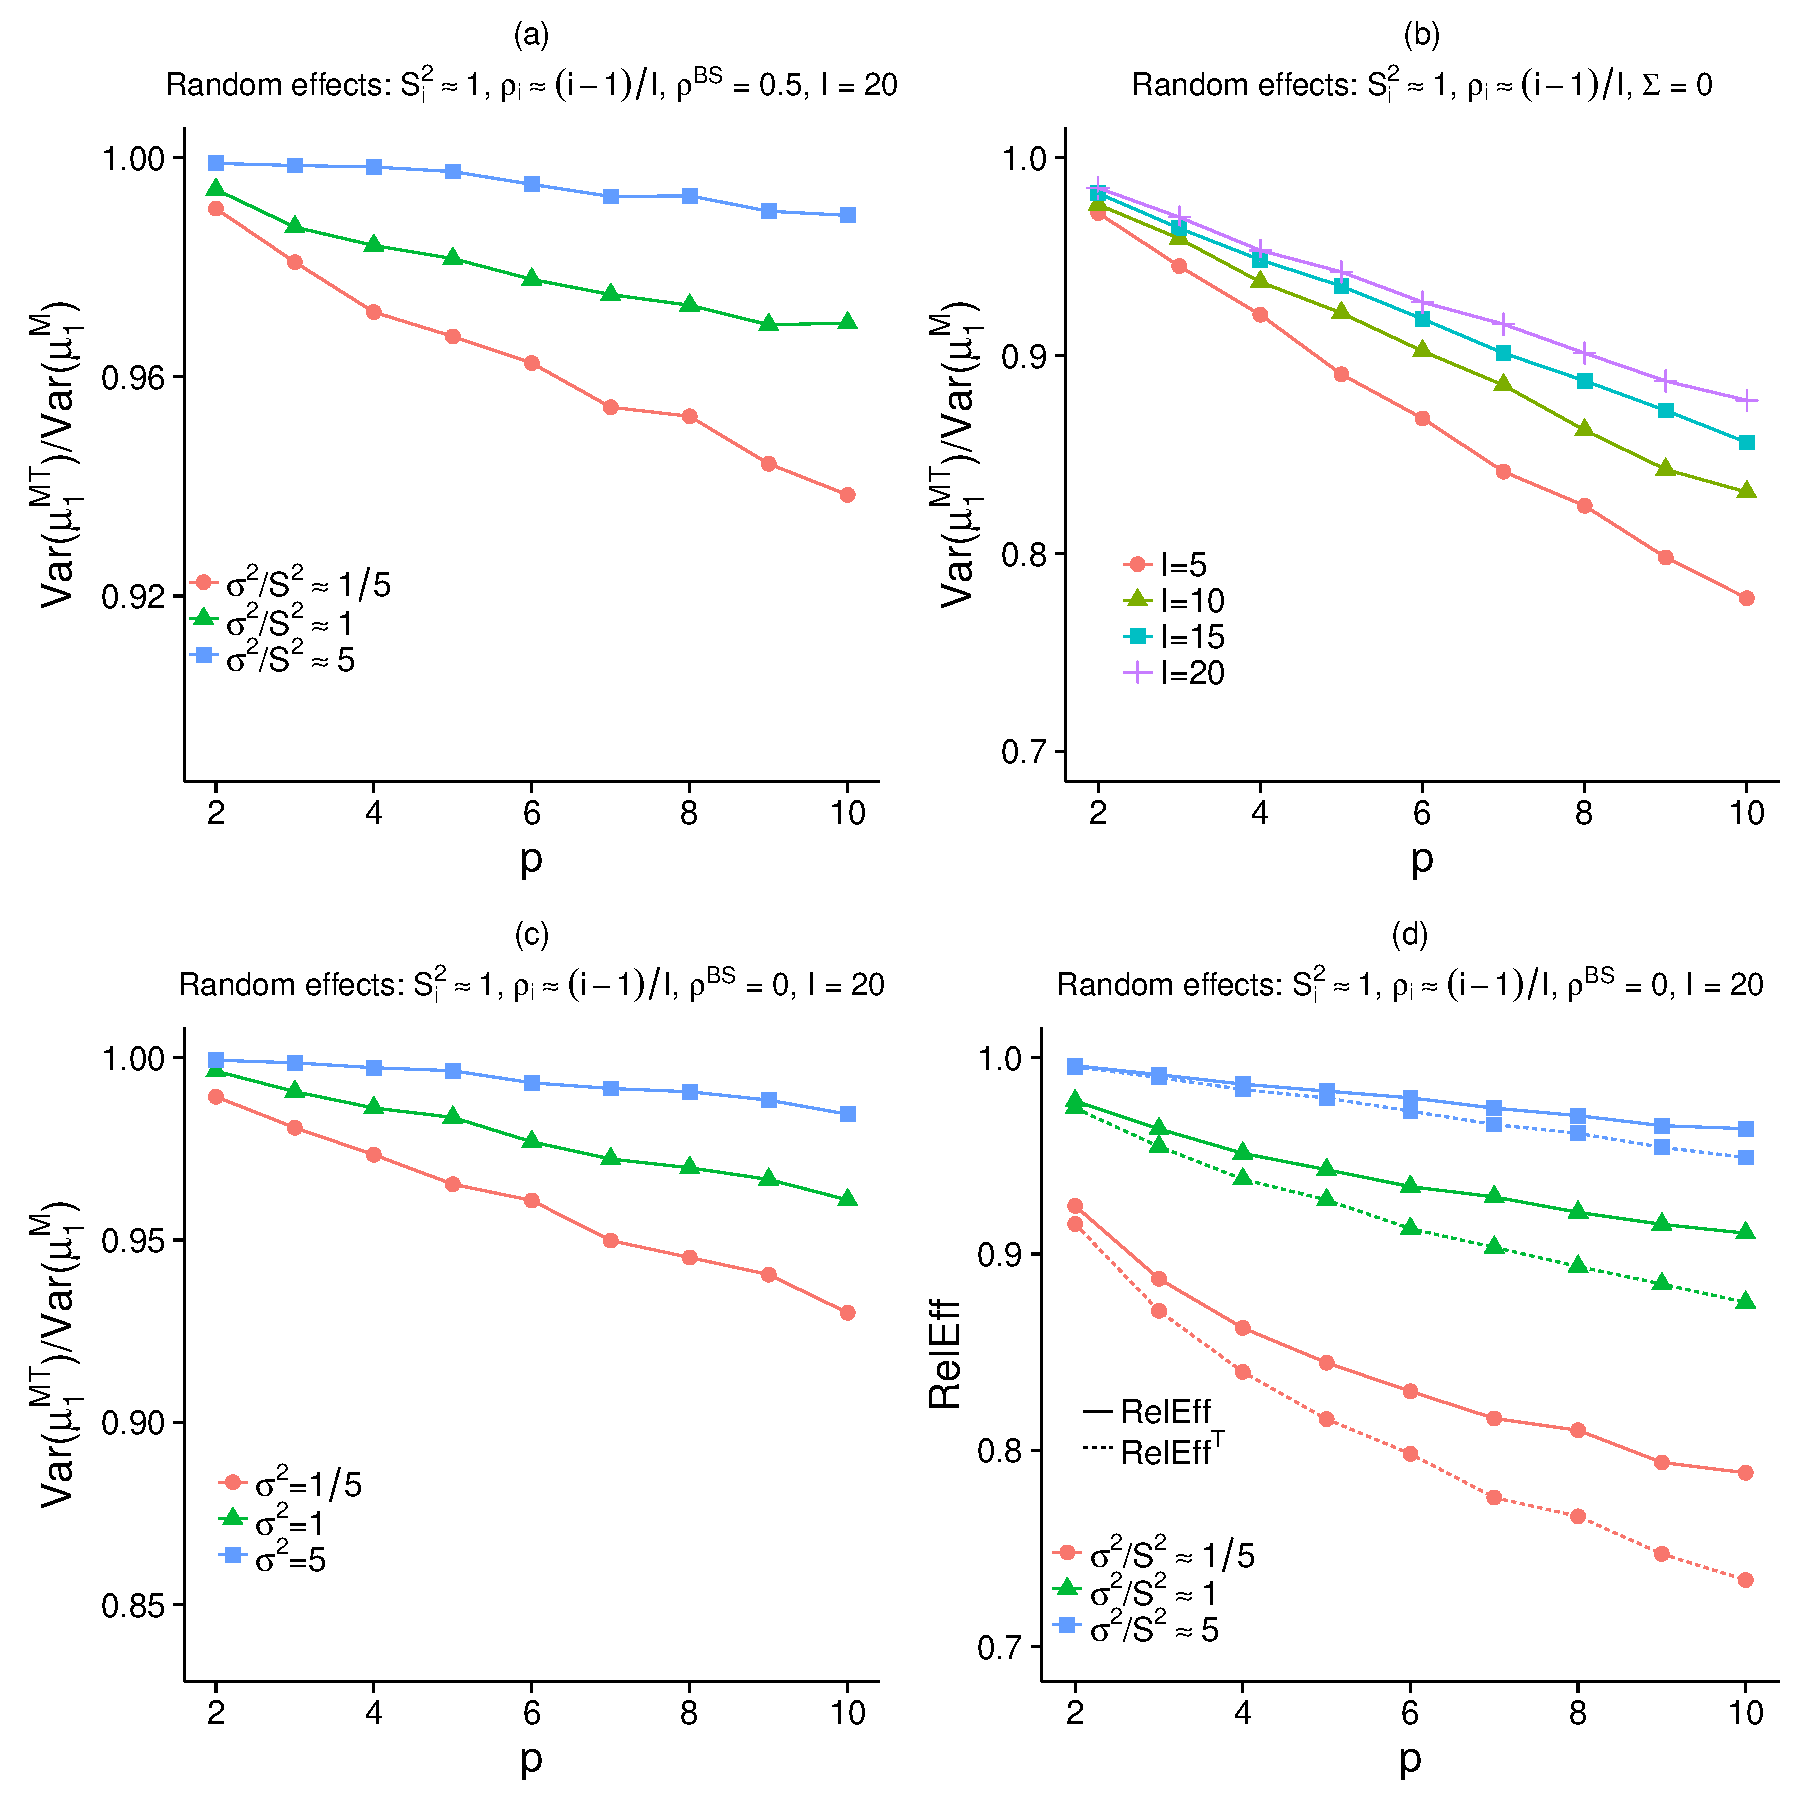
\includegraphics[width=\maxwidth]{figures/Figure_S3_panels_abcd-1} 

}



\end{knitrout}


\end{document}










